% !TEX encoding = Windows Latin 1


%
% Legt die Grundstruktur bzw. die Art des Dokuments sowie die Standardschriftgr"a"ae fest.
%
\documentclass[11pt]{article}

%
% Legt das Seitenlayout fest.
%
\usepackage[a4paper, margin=1.0in]{geometry}

%
% Legt die verwendete Schrift fest.
%
\usepackage{times}

%
% Legt die Worttrennungsregeln fest.
%
\usepackage[ngerman]{babel}

%
% Legt die Eingabekodierung fest.
%
\usepackage[latin1]{inputenc}
\usepackage[T1]{fontenc}

%
% Erm"aglicht die Darstellung von Farben sowie die Bezeichnung von Farben durch Namen.
%
\usepackage[usenames, dvipsnames]{color}

%
% Erm"aglicht das Einf"agen von Grafiken.
%
\usepackage{graphicx}

%
% Erleichtert die Darstellung von URLs.
%
\usepackage{url}

%
% Erlaubt die Bearbeitung von Bilder-, Diagramm- und Tabellenunterschriften.
%
\usepackage[hang, normalsize, bf]{caption}

%
% Legt fest, dass die AMS-Symbole benutzt werden.
%
\usepackage{amsmath}
\usepackage{amssymb}

%
% Erm"aglicht die Verwendung von vielen mathematischen Symbolen.
%
\usepackage{mathabx}

%
% Erm"aglicht die Verwendung der \today-Anweisung.
%
\usepackage[nodayofweek]{datetime}

% Erleichtert die Formattierung von Quelltexten.
\usepackage{listings}

%
% Erm"aglicht die einfachere Bearbeitung von Tabellen.
%
\usepackage{tabularx}

%
% Erm"aglicht die Darstellung von Tabellen auf mehreren Seiten (s. Dokumentation).
%
\usepackage{ltxtable}

%
% Erm"aglicht, Appendices in das Inhaltverzeichnis zu "abernehmen.
%
\usepackage[toc]{appendix}

%
% Erm"aglicht das Zusammenf"agen mehrerer Zeilen einer Tabelle.
%
\usepackage{multirow}
%
% Legt fest, welche Sprache in der Bibliographie verwendet werden soll.
%
%\usepackage[fixlanguage]{babelbib}

%
% Legt PDF-Format: PDF-A-1a fest
%
\usepackage[a-1a]{pdfx}

%%%%%%%%%%%%%%%%%%%%%%%%%%%%%%%%%%%%%%%%%%%%%%%%%%%%%%%%%%%%%%%%%%%%%%%%%%%%%%%%
%                                                                              %
% Einstellungen                                                                %
%                                                                              %
%%%%%%%%%%%%%%%%%%%%%%%%%%%%%%%%%%%%%%%%%%%%%%%%%%%%%%%%%%%%%%%%%%%%%%%%%%%%%%%%

%%%%%%%%%%%%%%%%%%%%%%%%%%%%%%%%%%%%%%%%%%%%%%%%%%%%%%%%%%%%%%%%%%%%%%%%%%%%%%%%
% einstellungen: url
%%%%%%%%%%%%%%%%%%%%%%%%%%%%%%%%%%%%%%%%%%%%%%%%%%%%%%%%%%%%%%%%%%%%%%%%%%%%%%%%

\urlstyle{tt}

%%%%%%%%%%%%%%%%%%%%%%%%%%%%%%%%%%%%%%%%%%%%%%%%%%%%%%%%%%%%%%%%%%%%%%%%%%%%%%%%
% einstellungen: bibliographie
%%%%%%%%%%%%%%%%%%%%%%%%%%%%%%%%%%%%%%%%%%%%%%%%%%%%%%%%%%%%%%%%%%%%%%%%%%%%%%%%

%\selectbiblanguage{german}
%\bibliographystyle{babplain}
\bibliographystyle{alpha}

%%%%%%%%%%%%%%%%%%%%%%%%%%%%%%%%%%%%%%%%%%%%%%%%%%%%%%%%%%%%%%%%%%%%%%%%%%%%%%%%
%                                                                              %
% ANWEISUNGEN                                                                  %
%                                                                              %
%%%%%%%%%%%%%%%%%%%%%%%%%%%%%%%%%%%%%%%%%%%%%%%%%%%%%%%%%%%%%%%%%%%%%%%%%%%%%%%%

\setlength{\parskip}{1.5ex plus 0.5ex minus 0.5ex}
\setlength{\parindent}{0em}

%%%%%%%%%%%%%%%%%%%%%%%%%%%%%%%%%%%%%%%%%%%%%%%%%%%%%%%%%%%%%%%%%%%%%%%%%%%%%%%%
% anweisungen: r"amische zahlen
%%%%%%%%%%%%%%%%%%%%%%%%%%%%%%%%%%%%%%%%%%%%%%%%%%%%%%%%%%%%%%%%%%%%%%%%%%%%%%%%

\makeatletter
\newcommand{\rmnum}[1]{\romannumeral #1}
\newcommand{\Rmnum}[1]{\expandafter\@slowromancap\romannumeral #1@}
\makeatother

%%%%%%%%%%%%%%%%%%%%%%%%%%%%%%%%%%%%%%%%%%%%%%%%%%%%%%%%%%%%%%%%%%%%%%%%%%%%%%%%
%                                                                              %
% DOKUMENT                                                                     %
%                                                                              %
%%%%%%%%%%%%%%%%%%%%%%%%%%%%%%%%%%%%%%%%%%%%%%%%%%%%%%%%%%%%%%%%%%%%%%%%%%%%%%%%


\begin{document}

\inputencoding{latin1}


%%%%%%%%%%%%%%%%%%%%%%%%%%%%%%%%%%%%%%%%%%%%%%%%%%%%%%%%%%%%%%%%%%%%%%%%%%%%%%%%
% dokument: titelblatt
%%%%%%%%%%%%%%%%%%%%%%%%%%%%%%%%%%%%%%%%%%%%%%%%%%%%%%%%%%%%%%%%%%%%%%%%%%%%%%%%

\begin{titlepage}

  %
  % university logo
  %

  \begin{flushright}
    
\includegraphics[scale=0.75, keepaspectratio=true]{data/fig/logo.pdf}
  \end{flushright}

  %
  % university, department & lecture info
  %

  \begin{center}
    \ \\
    \textsc{\Large
      Universit"at Potsdam, \\Institut f"ur Informatik \\
      \ \\
      \ \\
      Software Engineering, WiSe 2017-18 \\
      \ \\
      \ \\
      Projektarbeit -- Teil I \\
      Gruppe 5
      \ \\
      \ \\
    }
    {\huge \bfseries
      SharedBox Ultimate \\
    }
    \ \\
    \ \\
    \ \\
    \ \\
    \ \\
    \ \\
    \ \\

    %
    % author & supervisors
    %

    \large
    \begin{tabularx}{\textwidth}{ l X X }
      \emph{Autoren}:	&                   &	\emph{Betreuer}:        \\
                  	&                   &                           \\
      Marco Akrutat	& (Mat-Nr.\ 771933) &	Prof. Dr.\ Christian Hammer \\
      Marius Gerdes	& (Mat-Nr.\ 772451) &	M. Sc.  Sascha Gross \\
      Ariane M�ting	& (Mat-Nr.\ 775943) &	G�nther Wullaert  \\
      Sebastian Kunst	& (Mat-Nr.\ 781823) &	Juliane Scherlitzki    \\
      Aza Taha	& (Mat-Nr.\ 767351) &	 \\
    \end{tabularx}

    \vfill
    {\Large \today}
  \end{center}
\end{titlepage}

%%%%%%%%%%%%%%%%%%%%%%%%%%%%%%%%%%%%%%%%%%%%%%%%%%%%%%%%%%%%%%%%%%%%%%%%%%%%%%%%
% dokument: inhaltsverzeichnis
%%%%%%%%%%%%%%%%%%%%%%%%%%%%%%%%%%%%%%%%%%%%%%%%%%%%%%%%%%%%%%%%%%%%%%%%%%%%%%%%

\tableofcontents{}
\newpage{}

%%%%%%%%%%%%%%%%%%%%%%%%%%%%%%%%%%%%%%%%%%%%%%%%%%%%%%%%%%%%%%%%%%%%%%%%%%%%%%%%
% dokument: kapitel
%%%%%%%%%%%%%%%%%%%%%%%%%%%%%%%%%%%%%%%%%%%%%%%%%%%%%%%%%%%%%%%%%%%%%%%%%%%%%%%%

\section{Daten}

\subsection{Teilnehmer}

\begin{center}
\begin{tabular}{|c|c|c|c|}
\hline
\textbf{Name} &\textbf{Vorname} & \textbf{Position} &\textbf{intern/extern}\\\hline
Akrutat & Marco     & Full Stack Developer / Teamleader           & intern\\\hline
Gerdes   & Marius & Sen. Backend Developer          & intern \\\hline
M�ting & Ariane  & Sen. Frontend Developer         & intern \\\hline
Kunst  & Sebastian & Junior Frontend Developer       & intern\\\hline
Taha & Aza   & Werkstudent / Scrummaster           & intern\\\hline
Gro�  & Sascha & Leitender Endanwender & extern\\\hline
\end{tabular}
\end{center}

\section{Scope Management}

Das Projekt erfordert sowohl die Implementierung eines Front-Ends, welches als Eingabefl�che f�r die Benutzer dient, sowie die Implementierung des Back-Ends, dem eigentlichen Kernsystem. 

\begin{figure}[h]
\centering
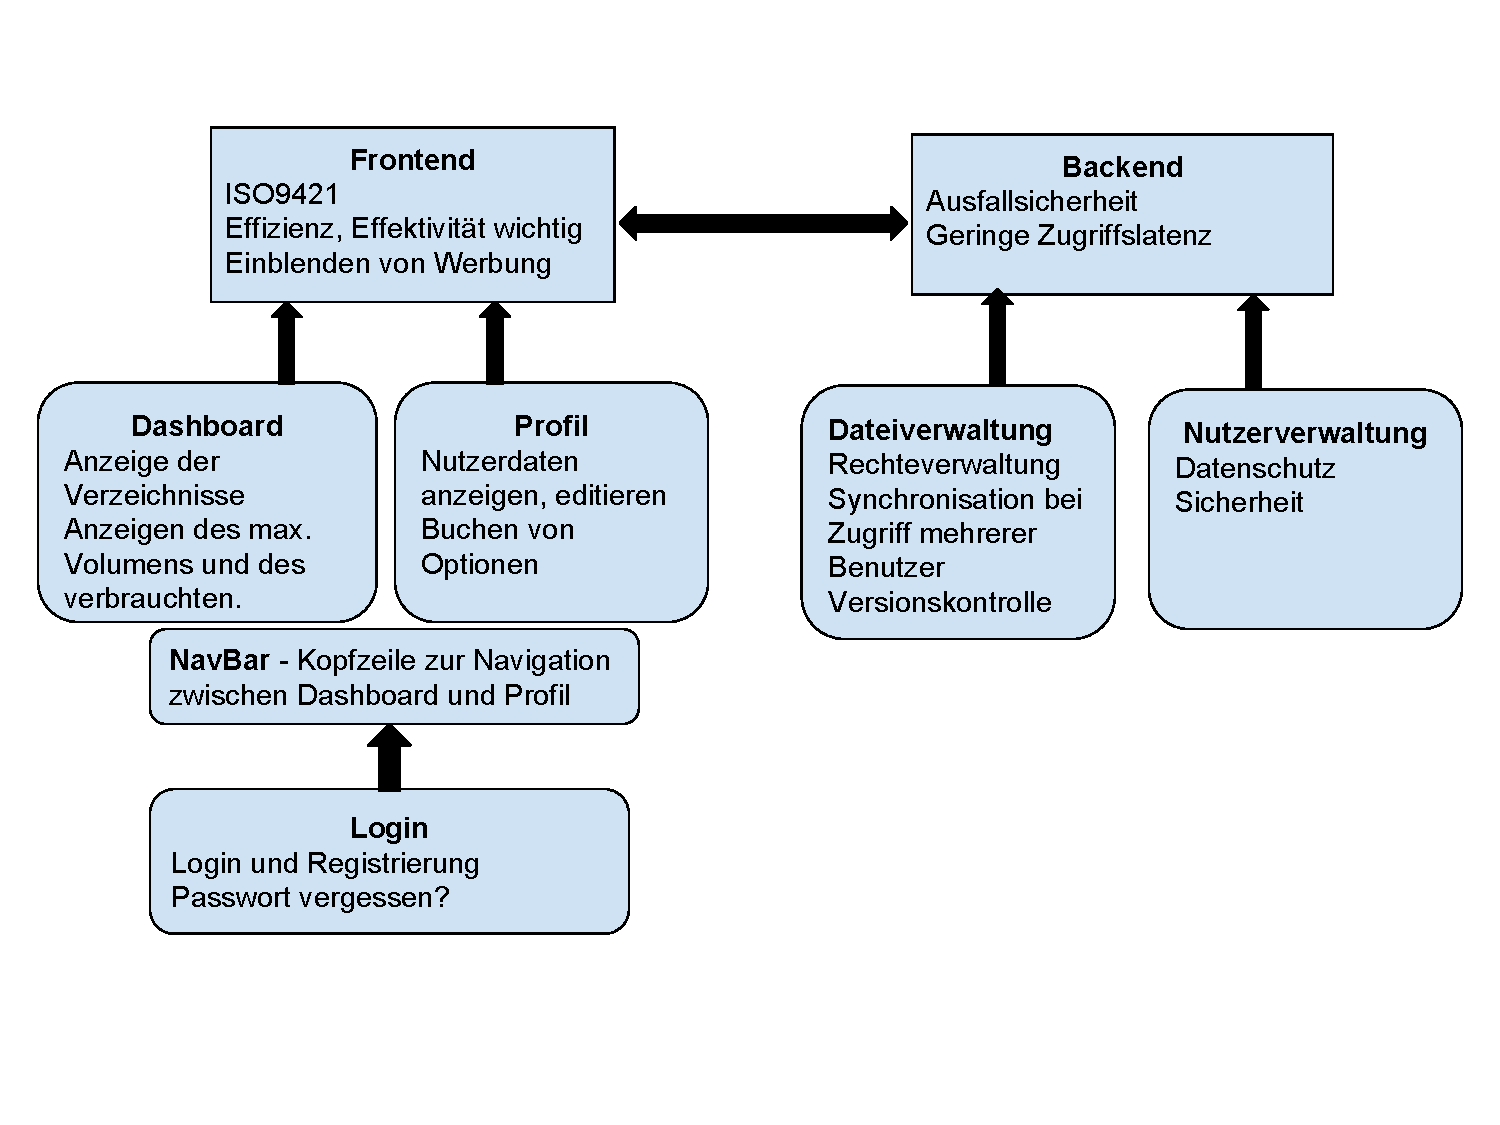
\includegraphics[page=1,width=\textwidth,height=.95\textheight,keepaspectratio] {ProjectStructure.pdf}
\caption{Work Breakdown Structure}
\end{figure}
\subsection{Aufgabendefinition}

Die Anforderungen an das Front-End sind eine hohe Effizienz, und Effektivit�t. Hierzu wird eine m�glichst intuitive Oberfl�che implementiert, die den Normen der ISO9421-Ergonomie der Mensch-System-Interaktion entspricht. Die Aufgaben sind hierbei Implementierung und Design des Loginportals, sowie des Dashboards und der Profilverwaltung. Hierbei wird Wert darauf gelegt f�r den Nutzer ansprechende Werbefl�chen zu schaffen, die die Funktionalit�t des Produktes nicht beeintr�chtigen.

Die Anforderungen an das Back-End sind unter anderem eine hohe Ausfallsicherheit, sowie eine geringe Zugriffslatenz. In der Nutzerverwaltung muss die Sicherheit der Daten gew�hrleistet werden. Im Bereich der Dateiverwaltung legen wir Wert auf eine reibungslose Synchronisation zwischen mehreren Benutzern. Die Implementierung einer primitiven Versionskontrolle wird ebenfalls umgesetzt.

Aus den Anforderungen ergibt sich die Work-Breakdown-Structure (s. Abbildung 1).

\section{Qualit"atsmanagement}

\subsection{Qualit"at Planung}

\subsection{Qualit"at Sicherung}

\subsection{Qualit"at Kontrolle}

\section{Personal Management}

Um einen m�glichst effektiven Einsatz der am Projekt beteiligten Entwickler zu gew�hrleisten, haben wir uns entschieden agil vorzugehen und nach Scrum zu entwickeln.

\subsection{Aufgabenverteilung}

Das Entwicklerteam f�r dieses Projekt besteht aus f�nf Leuten, vier Vollzeitangestellten Entwicklern und einem Werkstudenten in Teilzeit.
Als Full-Stack-Entwickler deckt unser Teamleiter beide gro�en Bereiche des Projektes ab. Im Bereich des Back-End und Front-End gibt es je einen erfahrenen Entwickler, unterst�tzt durch einen Berufseinsteiger im Bereich des Front-End und einen Werkstudenten im Bereich des Back-End.

Unser erfahrenener Back-End-Entwickler Marius Gerdes wird au�erdem die Rolle des Project Owners �bernehmen und den Kontakt mit dem Kunden pflegen.

Es wird in zwei-w�chigen Sprints gearbeitet und alle vier Wochen eine R�cksprache mit dem Kunden gehalten. Hierzu gibt es alle vier Wochen ein Dev-Fr�hst�ck, zu dem auch der Kunde eingeladen ist, bei dem die Projektteilnehmer in einer kurzen Pr�sentation erl�utern, welche Features sie implementiert haben, und wie sie dies taten. So hat jeder Entwickler einen Einblick in die Arbeit des anderen.

Um einen reibungslosen Ablauf der zwei-w�chigen Sprints zu gew�hrleisten gibt es zudem t�glich ein zehn-min�tiges Standup-Meeting, in dem jeder Entwickler vorstellen kann, was er am Vortag getan hat, welche Probleme auftraten, gegenfalls ob es eine L�sung gibt, und was er sich f�r den Tag vorgenommen hat. Dadurch ist jeder Entwickler im Bilde dar�ber, was die anderen gerade machen. Au�erdem kann man sich gegenseitig bei Problemen helfen, und Synergien werden so angeregt und gef�rdert.

\section{Time Management}

\subsection{Aufwandssch"atzung}

Eine Aufwandssch�tzung f�r das Projekt wurde mithilfe des intermediate COCOMO-Verfahrens durchgef�hrt. Das Projekt wurde als 'organic' eingestuft, auf etwa f�nf KDSI gesch�tzt und der Gesamtkostenfaktor M wie folgt ermittelt:\\\\
\texttt{
RELY 1.15 CPLX 0.85 TIME 1.11 ACAP 1 PCAP 1.17 LEXP 1.07 TOOL 1 SCED 1\\\\
M = 1.36\\\\}
Damit ergibt sich ein Projektaufwand von 23,6 Personenmonaten.
In Anbetracht der Ressourcen unseres Teams ergibt sich eine Projektdauer von etwa f�nfeinhalb Monaten. Das entspricht elf Sprints. Unser Full-Stack-Developer wird sicherstellen, dass die Projektdauer der Teilsysteme nicht zu stark von einander abweichen und das Gesamtprojekt im ermittelten Zeitrahmen bleibt.

Zeitlich wird das Projekt in f�nf Meilensteine gegliedert welche unterschiedliche Features enthalten. Jeder Meilenstein sollte etwa zwei Sprints in Anspruch nehmen (siehe Projektplan).

\subsection{Projektplan}

\begin{figure}[h]
\centering
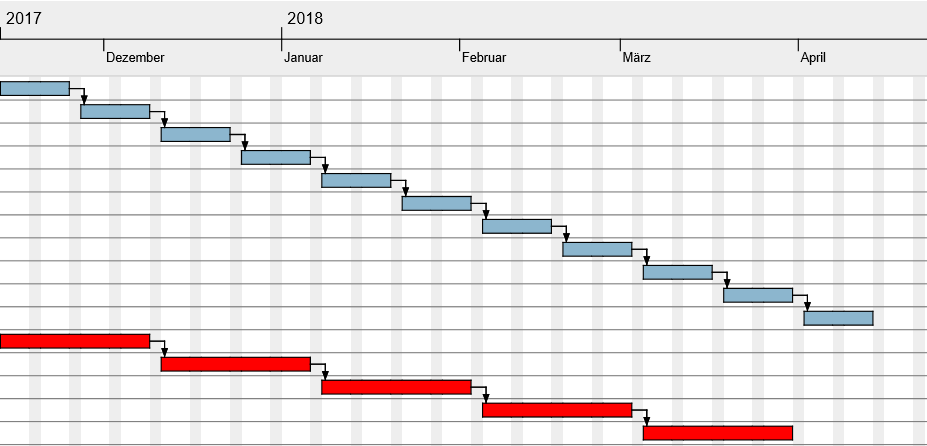
\includegraphics[page=1,width=\textwidth,height=.95\textheight,keepaspectratio] {gantt.png}
\caption{Gantt-Chart, Rot: Meilenstein, Blau: Sprint}
\end{figure}

\subsection{Soll/Ist Vergleich}

\section{Besonderheiten}

\subsection{Beziehungen zwischen den Aufgabenteilen}


\subsection{Externe Verz"ogerungen}


\section{Organisation}

\subsection{Abrechnung des Time- und Ressourcenmanagements}


\subsubsection{Stundenzettel}


\subsection{Kommunikations- und Toolplanung}

Wie bereits in der Sektion Personalmanagement erw�hnt gibt es ein t�gliches Standup-Meeting sowie ein monatliches Dev-Fr�hst�ck. Dar�ber gibt es eine Gruppe f�r das Projekt auf unserem firmeneigenen mattermost-Server, die zur weiteren Kommunikation innerhalb des Teams benutzt werden kann.
Zur Versionkontrolle wird ein Projekt in unserem Gitlab angelegt.

\subsection{Urlaub und Krankheit}


%%%%%%%%%%%%%%%%%%%%%%%%%%%%%%%%%%%%%%%%%%%%%%%%%%%%%%%%%%%%%%%%%%%%%%%%%%%%%%%%
% dokument: bibliographie
%%%%%%%%%%%%%%%%%%%%%%%%%%%%%%%%%%%%%%%%%%%%%%%%%%%%%%%%%%%%%%%%%%%%%%%%%%%%%%%%

\clearpage
\phantomsection
\addcontentsline{toc}{section}{Literatur}
\bibliography{swe1-projekt}



\end{document}